\documentclass[conference]{IEEEtran}

\usepackage{cite}
\usepackage{amsmath,amssymb,amsfonts}
\usepackage{algorithmic}
\usepackage{graphicx}
\usepackage{textcomp}
\usepackage{mathtools}
\usepackage{amsmath}
\usepackage{multirow}
\usepackage{algorithm}
\usepackage{algorithmic}
\usepackage{xcolor}
\usepackage{url}
\def\BibTeX{{\rm B\kern-.05em{\sc i\kern-.025em b}\kern-.08em
    T\kern-.1667em\lower.7ex\hbox{E}\kern-.125emX}}
\begin{document}


% Title Block

\title{Genetic Programming with Rademacher Complexity for Symbolic Regression}


% Author Block
\author{\IEEEauthorblockN{Christian Raymond, Qi Chen, Mengjie Zhang, Bing Xue}
\IEEEauthorblockA{\textit{School of Engineering and Computer Science} \\
\textit{Victoria University of Wellington,}
Wellinton, New Zealand \\
christianfraymond@gmail.com, \\\{Qi.Chen, Mengjie.Zhang, Bing.Xue\}@ecs.vuw.ac.nz}
}

\maketitle


% Abstract Block

\begin{abstract}
Genetic Programming (GP) for symbolic regression is often prone to overfitting the training data, causing poor performance on unseen data. A number of recent works in the field have been devoted to regulating this problem by investigating both the structural and functional complexity of GP individuals during the evolutionary process. This work uses the Rademacher complexity and incorporates it into the fitness function of GP, utilising it as a means of controlling the functional complexity of GP individuals. The experiment results confirm that the new GP method has a notable generalization gain compared to the standard GP and Support Vector Regression (SVR) in most of the considered problems. Further investigations also show that the new GP method generates symbolic regression models that could not only release the overfitting trend in standard GP but also are significantly smaller in size compared to their counterparts in standard GP.
\end{abstract}


% Key Words Block

\begin{IEEEkeywords}
genetic programming, symbolic regression, generalization, structural risk minimization, rademacher complexity
\end{IEEEkeywords}


% Key Words Block

\section{Introduction}

In machine learning, a class of algorithms called supervised learners seek to learn from and make predictions on labelled data by mapping the inputs $X$ to the outputs $Y$, where $X$ and $Y$ are drawn on the assumption of a joint probability distribution $P(X, Y)$. In the simplest case, this data is partitioned into two sets: a training set which is given to a learning algorithm for learning a model, and an unseen test set which is used to verify the learnt models on unseen data.

Unfortunately, the joint probability distribution $P(X, Y)$ is typically unknown thus a hypothesis/candidate solution must be selected based on the empirical risk minimization (ERM) principle \cite{b13}, which states that the hypothesis that minimizes the empirical risk, i.e. the training error, is the optimal hypothesis. However, this leaves a learner susceptible to the common problem of overfitting, which is prevalent in all supervised learning algorithms. Overfitting is where the algorithm fits the training data too closely, making it unable to generalize well on the unseen data i.e. the test set \cite{b1}.

Instead of using the ERM principle, machine learning research has progressively utilized the powerful structural risk minimization (SRM) framework developed in the field of learning theory \cite{b2}. SRM seeks to incorporate the use of a regularization penalty to help manage the complexity of candidate solutions, which in turn results in less overfitting and better generalization of the learnt classifier/model on the unseen data.

In Genetic Programming (GP) \cite{b3} for symbolic regression \cite{b4}, a number of candidate solutions are developed through simulating evolution to generate the optimal hypothesis, which maps the input variables to the output variables. The evolutionary process is traditionally guided through giving propagation rights to the hypothesises i.e. candidate solutions, that have the lowest training error i.e. the ERM framework, which makes GP prone to overfitting.

There have been a few works recently which have applied the SRM framework to GP with very promising results such as: \cite{b5} and \cite{b17} which use the Vapnik-Chervonenkis dimension (VC-dimension) for estimating the difference between the generalization error and the empirical error, and \cite{b6} which uses the order of non-linearity to quantify the complexity of a hypothesis. Nonetheless, the topic of model complexity in GP for symbolic regression has certainly not received the appropriate attention that it deserves. 

Based on what has been stated earlier, this paper aims to develop a new GP for symbolic regression method that uses the SRM framework to regulate the model complexity of the solutions generated in the evolutionary process. This will be done by introducing a new fitness function  which takes both the training error and the Rademacher complexity of a hypothesis into account. 

In computational learning theory, the Rademacher complexity \cite{b26} \cite{b27} is a modern distribution dependent measure for the complexity of a hypothesis, which can be applied to learning algorithms to approximate the performance of a learned hypothesis on unseen data (test set). Since the Rademacher complexity is a distribution dependent complexity measure, for a specific input distribution, it can often give tighter generalization bounds (especially so for the average case)  than other complexity measures such as the VC-dimension which is distribution independent.

The Rademacher complexity has been successfully used to regulate supervised learning algorithms in a small number of cases such as \cite{b11} and \cite{b12}, however this will be its first application to GP. The new method developed is expected to produce significantly functionally and structurally simpler, less complex models which can generalize better onto unseen data. 

\bigbreak
Specifically, this research has three key objectives:

\begin{itemize}

  \item to use the Rademacher complexity to measure the functional complexity of GP individuals and investigate whether it can accurately reflect the generalization performance of GP individuals.
  
  \item to propose a new fitness function in GP for symbolic regression which can drive the evolutionary process towards individuals that have better generalization capacity by incorporating the Rademacher complexity of GP individuals.
  
  \item to investigate whether the newly proposed GP method can lead to the development of more compact individuals compared to the standard GP.

\end{itemize}

\subsection{Organisation}
The remainder of this paper is organized as follows. Section \ref{se:bg} presents a brief review on the related work. Section \ref{se:method} presents the design of the proposed method. This is followed by an introduction of the benchmark problems and experiments in Section \ref{se:exp}. Results and discussions are presented in Section \ref{se:Results} and finally the conclusion and future work are given in Section \ref{se:conclu}.


\section{Background}
\label{se:bg}

\subsection{Genetic Programming for Symbolic Regression}

Genetic Programming (GP) is a stochastic population-based metaheuristic optimization algorithm from the field of Evolutionary Computation (EC). GP simulates Darwinian evolution through the use of genetic operators such as crossover, mutation, elitism and selection to evolve a population of individuals (hypothesises). In GP, the individuals are traditionally represented as expression trees and are given a fitness score based on how well they accomplish one or more of the target objective. 


This work focuses on tackling the task of symbolic regression, which is a kind of regression analysis, seeking to estimate the underlying relationship between the input (independent) variables and the output (dependent) variables expressed as mathematical model/functions. GP is a good approach to symbolic regression due to its ability to build a large number of potential models in a single execution and its ability to produce these models without any underlying assumptions about the distribution of the data and the model structure. A large number of researches have been devoted to make GP a more suitable approaches to symbolic regression \cite{b16,b17,b18,b19}.

\subsection{Model Complexity and Generalization in GP}

Model Complexity is an important topic in GP for symbolic regression for a number of reasons. The first being that too simple of a model may produce poor predictive performance, while a highly complex model may be prone to overfitting the training data causing a degradation of accuracy on the test set (unseen data) often referred to as having a high generalization error.

Learning algorithms such as GP are evaluated based on a finite sample, as a result the performance evaluation may be sensitive to sampling error, often made more apparent as the number of training instances decreases. This means that the performance evaluation provided against the training set may not necessarily provide much information about the performance of GP on unseen data. To minimize the generalization error and maximize performance in GP overfitting must be regulated carefully.

In GP, high model complexity is also responsible for bloat, where there is an excessive code growth/structural complexity in the expression tree without a corresponding improvement in the individual's fitness \cite{b7}. High structural complexity is computationally more expensive to evaluate and is harder to interpret, making it not pragmatic in many commercial contexts.

For many years, researchers have investigated the link between the performance of GP and structural complexity, examples of this being the various approaches of parsimony pressure \cite{b8}\cite{b9}. However, it should be noted that a large expression tree is not equivalent to a high functional complexity, especially since many expression trees in symbolic regression could be algebraically simplified, reducing the structural complexity without changing the functional complexity. Furthermore, recent contributions to the field show that eliminating bloat does not necessarily eliminate overfitting on the unseen data \cite{b10}. 

\subsection{Rademacher Complexity}

The Rademacher complexity in its simplest form can be considered as the ability for a hypothesis to fit random noise. If a hypothesis can fit the random noise with a high degree of accuracy, the hypothesis is of a high complexity. In contrast to this, if a hypothesis cannot fit the random noise, it is of a low complexity. Explicitly, the Rademacher complexity can be defined using a simple case of a binary classification problem. We begin by first defining a training set \textit{S}: 
\begin{equation}
\footnotesize
	S = ((x_{1} y_{1}),(x_{2}, y_{2}) \dots (x_{m}, y_{m})) \;where\; y_{i} = \{-1, +1\}\nonumber.
\end{equation}
Then define a hypothesis such that \textit{h}:
\begin{equation}
\footnotesize h(X) \rightarrow \{-1, +1\}\nonumber
\end{equation}
To access how accurately \textit{h} classifies \textit{S}, let the following set of equations provide an alternative definition of the training error attained by $h$ on $S$.
\begin{equation}\label{training_error}
\footnotesize
\begin{aligned}
\hat{err(h)} 
& = \frac{1}{m}\sum\limits_{i=1}^m 1 \{h(x_{i}) \neq y_{i}\}\\
& = \frac{1}{m}\sum\limits_{i=1}^m
	\begin{cases}
    1, & \text{if $\left(h(x_{i}\right), y_{i}) = (+1,-1)\;or\;(-1,+1)$}\\
    0, & \text{if $\left(h(x_{i}\right), y_{i}) = (+1,+1)\;or\;(-1,-1)$}
	\end{cases}\\
& = \frac{1}{m}\sum\limits_{i=1}^m \frac{1 - y_{i}h(x_{i})}{2}\\
& = \frac{1}{2} - \frac{1}{2m}\sum\limits_{i=1}^m y_{i}h(x_{i})
\end{aligned}
\end{equation}

\bigbreak
Using this alternative definition of the training error stated in \eqref{training_error}, we can subsequently define: 
\begin{equation}\label{cor}
\footnotesize
correlation = \frac{1}{m}\sum\limits_{i=1}^m y_{i}h(x_{i})
\end{equation}

The $correlation$ can be considered to be the correlation of the prediction $h(x_{i})$ on labels in the training set $y_{i}$. If $h(x_{i})$ and $y_{i}$ are always the same (all correct classification), the correlation is equal to $1$, and if they always disagree (all incorrect classification) then the correlation is equal to $0$.
Thus when searching for the optimal hypothesis i.e. the hypothesis that minimizes the training error, we can also alternatively search for the hypothesis such that \textit{h} satisfies:
\begin{equation}\label{best_hypothesis}
\footnotesize
	\max_{h} \frac{1}{m} \sum\limits_{i=1}^m y_{i}h(x_{i}),
\end{equation}
since the hypothesis \textit{h} that minimizes the training error is also the hypothesis that maximizes the correlation.


The Rademacher complexity extrapolates from what has been stated prior to modify the formula described in \eqref{best_hypothesis}, replacing the true label $y_{i}$ with a \textit{Rademacher random variable} denoted by $\sigma_{i}$ where: 

\begin{equation}\label{random_vector}
\footnotesize
	\sigma_{i}\begin{cases}
    +1, & \text{with probability = 0.5}\\
    -1, & \text{with probability = 0.5}
	\end{cases}
\end{equation}

The definition of the Rademacher complexity is given as follows:
\begin{equation}\label{rademacher}
\footnotesize
	Rad(h) = \max_{h} \frac{1}{m} \sum\limits_{i=1}^m \sigma_{i}h(x_{i})
\end{equation}

Here, the Rademacher complexity is equal to the maximum correlation that could be achieved when $h(x_{i})$ is compared to $\sigma_{i}$. A hypothesis \textit{h} that can attain a high correlation with $\sigma_{i}$ is of a high complexity, while a hypothesis \textit{h} that has a low correlation with $\sigma_{i}$ is of a low complexity and will often be able to generalize better onto unseen data. The generalization error bounds based on the Rademacher Complexity \cite{b26} can be giving by the formula:

\begin{equation}\label{bounds}
\footnotesize
 E[h]\leq\hat{E}_{S}[h] + 2Rad(h) + O\left(\sqrt{\frac{ln\left(1/\delta\right)}{m}}\right)
\end{equation}

The Rademacher complexity generalization error bounds provides a theorem which states that with a high probability i.e. $p \geq 1 - \delta$, the generalisation performance of a set of functions defined by $h$ is bounded by the training performance and the Rademacher complexity.


% Proposed Method Block

\section{The Proposed Method}
\label{se:method}
This work aims to introduce the Rademacher complexity into GP for symbolic regression to measure the complexity of the candidate solutions throughout the evolutionary process. The proposed method is named Genetic Programming with Rademacher Complexity (GPRC). GPRC is most notably different from standard GP in the fitness function which takes into account both the training error and the prospective models complexity.

\subsection{Introducing Rademacher Complexity to GP}

In standard GP for symbolic regression, typically the ERM framework is used, and has the following fitness function:
\begin{equation}\label{fitness_old}
\footnotesize
Fitness(h) = \hat{E}_{S}[h]
\end{equation}
where $\hat{E}_{S}[h]$ denotes the error of $h$ on $S$, which is computed using a performance metric such as: mean absolute error (MAE), mean square error (MSE) and root mean square error (RMSE). In GPRC, instead of using the equation given in \eqref{fitness_old}, the Rademacher bound formula defined in \eqref{bounds} is to be used, which will provide an estimation of the generalization/test errors of the candidate solutions throughout the evolutionary process. Note that the right portion of the formula in \eqref{bounds} is discarded since this would just introduce a constant penalty across all individual thus making it a redundant element. Thus, the generalization bound can be simplified to:

\begin{equation}\label{fitness_new}
E[h]\leq \hat{E}_{S}[h] + 2Rad(h)
\end{equation}

\bigbreak
\noindent
where the output of $2Rad(h)$ gives the correlation of $h$ on $\sigma$, which lies between the range of $(0, 1)$. Therefore it is desirable to have a performance metric such that $\hat{E}_{S}[h]$ does not dominate $2Rad(h)$, and ideally it would sit within the range $(0, 1)$. A straightforward solution is scaling the $\hat{E}_{S}[h]$, however simply scaling the $\hat{E}_{S}[h]$ by the range of the individuals in the population is problematic due to extreme outliers which will skew the $\hat{E}_{S}[h]$ and cause fluctuations in the fitness values across generations. To resolve this problem, the preferred performance metric to compute $\hat{E}_{S}[h]$ should be the relative squared error (RSE) defined below in \eqref{rse}. As the vast majority of models with a high predictive power have a RSE in the proximity of 1. Additionally it is a consistent performance metric which can be used across all generations.

\begin{equation}\label{rse}
\footnotesize
RSE = \hat{E}_{S}[h] = \frac{\sum\limits_{i=1}^m\left(\hat{y_{i}} - y_{i}\right)^2}{\sum\limits_{i=1}^m\left(\bar{\mathbf{y}} - y_{i}\right)^2}
\end{equation}

\bigbreak
For obtaining $Rad(h)$, it is desirable to take the average over a number of observations to give an accurate estimation of the complexity of $h$ on the average case. This would give the following updated equations shown in \eqref{compexity}, where $n$ is the number of observations/instances taken, and $m$ is the size of the training set, i.e. $|S|$.

\begin{equation}\label{compexity}
\footnotesize
\begin{aligned}
Rad(h) & =  \frac{1}{m}\left(\frac{1}{n}\sum\limits_{j=1}^n\left(\sum\limits_{i=1}^m \sigma_{i}h(x_{i})\right)\right)\\
&= \frac{1}{m}\left(\frac{1}{n}\sum\limits_{j=1}^n\left(\sum\limits_{i=1}^m \begin{cases}
    1, & \text{if $h(x_{i}) \neq y_{i}$}\\
    0, & \text{if $h(x_{i}) = y_{i}$}
	\end{cases}\right)\right)\\
\end{aligned}
\end{equation}

\bigbreak
The original method to measure the Rademacher complexity has been used for a binary classification problem such that $h = X \rightarrow \{-1, +1\}$. To extend this method to symbolic regression where the output is continuous, the output needs to be converted to a binary value. To achieve this the following formula is applied, which normalizes each of the predictions $h(x_{i})$ by the \textit{range} of all the predictions made by $h$ on $S$:
\begin{equation}\label{regression}
\footnotesize
h(x_{i})\begin{cases}
    +1, & \text{when $(h(x_{i})$ / $range$) $\geq 1$}\\
    -1, & \text{when $(h(x_{i})$ / $range$) $< 1$}
\end{cases}
\end{equation}

Note that in the special case that $h$ has no range, i.e. when the output of $h$ is constant across all inputs, either +1 or -1 may be assigned.

Moreover, since the Rademacher complexity is a data dependent generalization bound, the optimal proportionate impact made by both the training error $\hat{E}_{S}[h]$ and the models complexity given by $Rad(h)$ will differ across different datasets depending on where in the solution space the best solution lies. Therefore two parameters are introduced, giving the new fitness function as follows:

\begin{equation}\label{fitness_final}
\footnotesize
Fitness(h) = \hat{E}_{S}[h] + \alpha\cdot\frac{\#gen}{\#maxgen} \cdot Rad(h)
\end{equation}
where the new parameters $\alpha$ and $\frac{\#gen}{\#max gen}$ are used to regulate the impact made by the hypothesis's complexity given by $Rad(h)$. Too much emphasis on minimizing the complexity can prevent the discovery of more complex yet more accurate solutions, thus it is sensible to parametrizing the function as a control mechanism. The value of the parameter $\alpha$ is problem dependent, for problems where GP has an obvious trend of overfitting, the complexity measure will give higher pressure through the use of a larger value of $\alpha$.

In the parameter $\frac{\#gen}{\#maxgen}$, $\#gen$ refers to the index number of the current generation and $\#maxgen$ is the maximum number of generations for the evolutionary process. This parameter was added so that there would be an increased focus on complexity in subsequent generation (since overfitting is often more likely to happen in later generations) without putting to much pressure on earlier generations and causing premature convergence.

This new fitness function in GPRC for symbolic regression is expected to guide the evolutionary process toward models which can achieve better generalization onto the unseen data in regards to the error. In contrast, the classic GP fitness function described in \eqref{fitness_old} which often overfits $S$. Furthermore, the models produced should have a lower complexity, resulting in smaller expression trees being produced at each generation.

\subsection{Implementing Rademacher Complexity in GP}

Fig.\ref{fig:evaluation} shows the implementation of the newly defined fitness function in GPRC, which is straightforward and does not require many alterations. At the start of each generation (before fitness evaluations occur) $n$ Rademacher random vectors (e.g. $\sigma = [-1, 1, \cdots, |S|]$) need to be generated, i.e. creating the random noise. This is done by creating $n$ number of arrays of size $m$, i.e. the number of instances in the training set $S$, populated with -1 and +1 values as per the formula \eqref{random_vector}. Note that these Rademacher random vectors are then reused across all fitness evaluations in the current generation for consistency. Given these Rademacher random vectors the detailed procedure for computing the fitness value of a single individual $h$ is given as follows:

\begin{enumerate}

  \item Calculate the relative squared error (RSE) defined in equation \eqref{rse} of the candidate solution on the training set $S$. At this stage, a record of all the predictions made by $h$ is to be kept.
  
  \item Iterate over the recorded list of predictions made in step $1)$, converting the output of $h$ to binary using the formula described in equation \eqref{regression}.
  
  \item Compute the average Rademacher complexity using the equation described in equation \eqref{compexity} using the recorded list of predictions made in the step $1)$ and the Rademacher random vectors generated at the start of the generation.
   
  \item Finally, calculate and set the fitness value of the candidate solution $h$ using the equation described in equation \eqref{fitness_final} using the RSE calculated in step $1)$, the Rademacher complexity calculated in step $3)$, the $\frac{\#gen}{\#max gen}$, and some predefined values of $\alpha$ set prior to execution.
  
\end{enumerate}

\begin{figure}[!ht]
\centerline{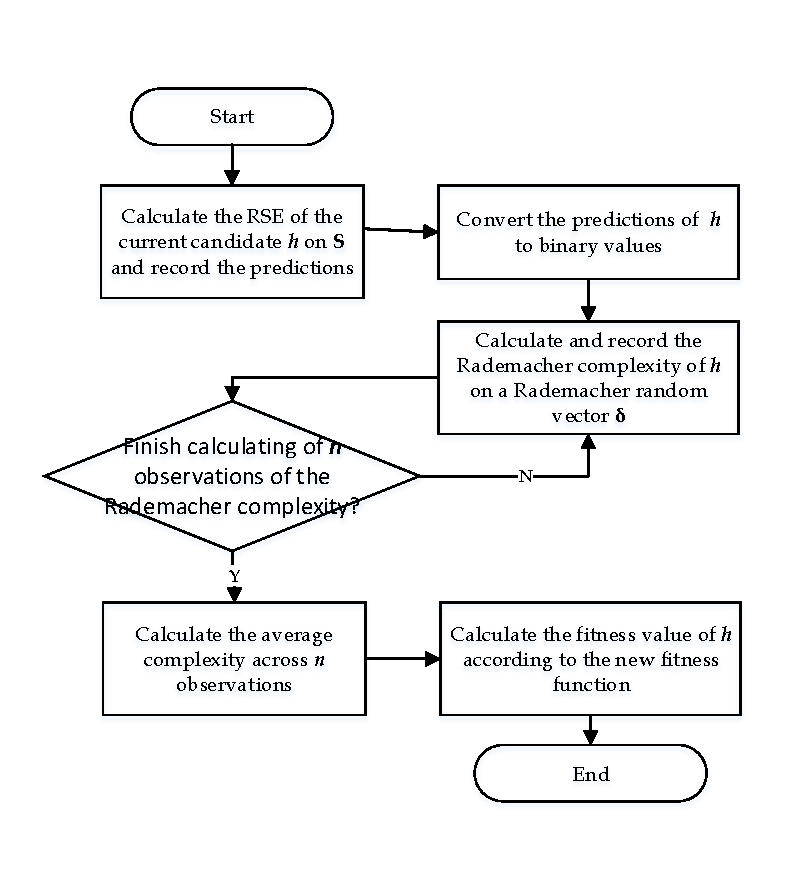
\includegraphics[height=9cm, width=8cm]{evaluation}}
\caption{Flowchart demonstrating the evaluation of one GP individual $h$ in GPRC}
\label{fig:evaluation}
\end{figure}


% Experimental Setup

\section{Experiment Settings}
\label{se:exp}

To investigate the generalization performance of GPRC for symbolic regression, a set of experiments have been conducted to compare it with two benchmark methods.
They are:

\begin{itemize}
	\item Standard Genetic Programming (\textit{GP}) and 
	\item Support vector regression (\textit{SVR}), which is a powerful regression method. The performance of SVR with a popular kernel function \textemdash{the radial basis function} is used as a baseline method for comparison.  
\end{itemize}

\subsection{Benchmark Problems}

\begin{table}[!ht]
	\scriptsize
	\caption{Number of features and instance in datasets}
	\label{tab:realworlddatasets}
	\centering
\begin{tabular}{|l|c|c|c|c|}
\hline
\multirow{2}{*}{} & \multirow{2}{*}{Features} & \multicolumn{3}{c|}{Instances} \\ \cline{3-5} 
                  &                           & Total   & Training  & Testing  \\ \hline
Concrete          & 8                         & 1030    & 309       & 712      \\
LD50              & 626                       & 234     & 71        & 163      \\
Wine              & 11                        & 1599    & 480       & 1119     \\
CCUN              & 122                       & 1994    & 199       & 1795     \\
DLBCL             & 7399                      & 240     & 160       & 80       \\ 
BHouse            & 13                        & 506     & 152       & 354      \\ 
\hline
\end{tabular}
\end{table}

As of currently there is no established suit of benchmarks which is specifically designed for testing the model complexity of GP for symbolic regression, following previous research on GP for symbolic regression \cite{b7, b17},  six symbolic regression datasets are taken from previous research and the University of California Irvine's (UCI) Machine Learning Repository \cite{b21}. The detailed information of the six datasets is summarized in Table \ref{tab:realworlddatasets}. The first four datasets are taken from UCI. The last two datasets median lethal dose (LD50) \cite{b22} and  Diffuse Large B-Cell Lymphoma (DLBCL) \cite{b23} are taken from previous research on regression.

Note that for the DLBCL dataset it was already pre-partitioned into training and testing sets, so in this work these sets were preserved. For the rest of the datasets which were not pre-partitioned, they were split into training and testing sets using $0.3/0.7$ respectively. The number of training instances are deliberately designed to be small for these problems, which is to simulate the real-world situation where there is not enough training instances available and the learning methods are more likely to be prone to overfitting. 

\subsection{Parameters Settings}
The default parameter settings for both standard GP and GPRC can be found in Table II, which defines the typical parameters required to execute GP. For GP with Rademacher Complexity there were some additional parameters to define. For the number of Rademacher complexity observations $n$ is set to $20$ which is the same value used in \cite{b15}. 


All the GP methods are implemented under the ECJ GP framework \cite{b24}. SVR is implemented under the R packages ``e1071'' \cite{b25} using the RBF kernel function and some other default settings.

\begin{table}[!ht]
\caption{Genetic Programming Parameters}
\begin{center}
\begin{tabular}{|l|l|}
\hline
\textbf{Parameter}    & \textbf{Value} \\ \hline
Number of Independent Runs  & 100       \\ \hline
Population Size       & 1024            \\ \hline
Number of Generations & 100            \\ \hline
Crossover Rate        & 0.9            \\ \hline
Mutation Rate         & 0.1            \\ \hline
Elitism         & top 10 individuals            \\ \hline
Fitness Function      & RSE            \\ \hline
Primitive Set         & $+$, $-$ , $\times$, $\div$ (protected)   \\ \hline
Maximum Tree Depth    & 11             \\ \hline\hline
$n$ (number of observations) & 20\\\hline
$\alpha$ (complexity pressure) & $2$ for LD50 and DLBCL \\
&$1$ for the others\\\hline
\end{tabular}
\end{center}
\end{table}

% Results and Discussion block

\section{Results and Discussion}
\label{se:Results}
The distribution of the training and test performance (RSE's) of the best-of-run models in GP and GPRC over 100 independent runs is shown in Fig. \ref{fig:Box}. Each method has two boxes and whiskers. The left one (red) is for the training performance and the right one (green) shows the test performance.  Since SVR is a deterministic method and can only obtain a single result, these results were shown using lines, where the red solid line shows the training performance and the green slashed line is for the test performance. The non-parametric statistical significance test, i.e. Wilcoxon test, with a significance level of 0.05, is conducted to compare the training RSEs and test RSEs of the best-of-run models between each of the two GP methods.  Z-test is employed to test whether there is any significant difference between the two GP methods (with 100 observations) and SVR (with a single observation).

\subsection{Comparing the Training Performance}

\begin{figure*}[h]
	\centering
	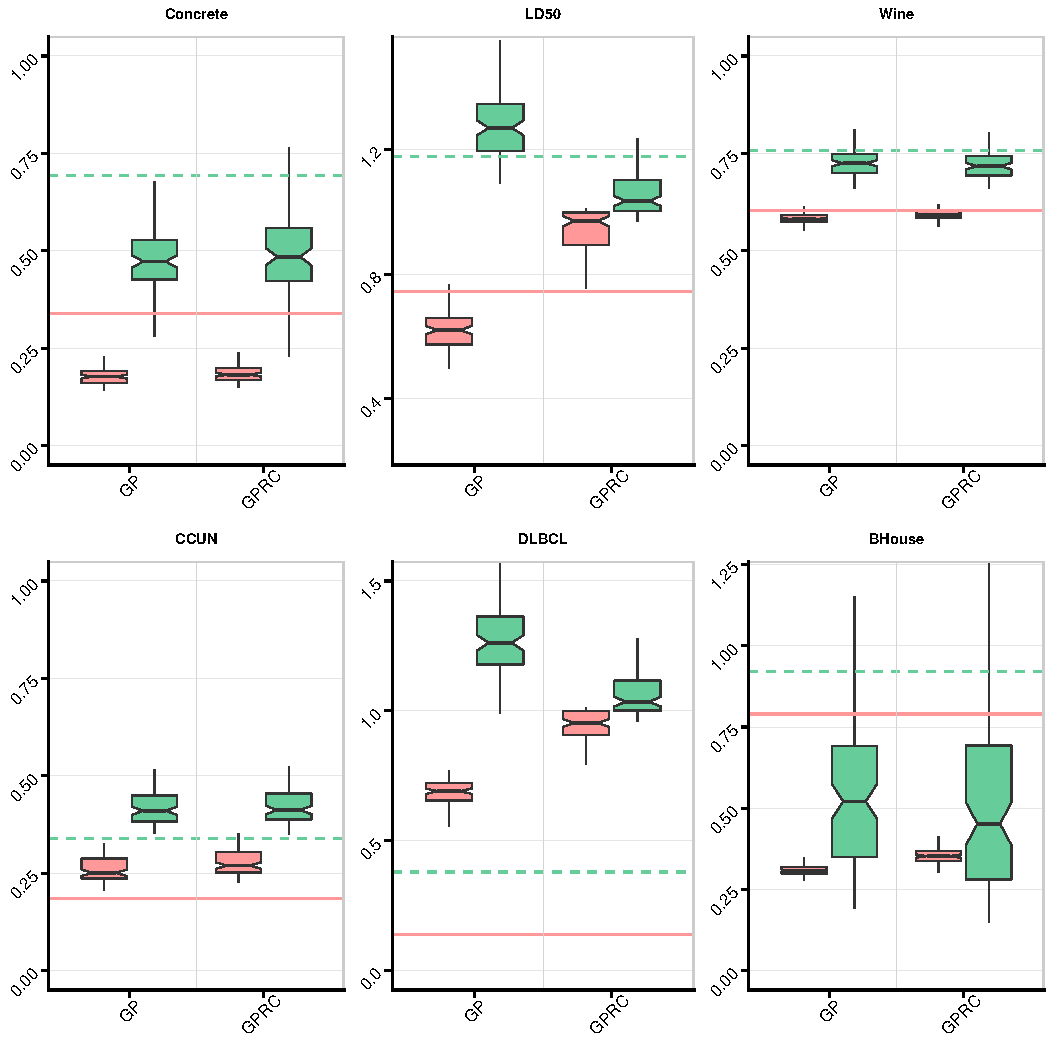
\includegraphics[height=11cm, width=13cm]{Box}
	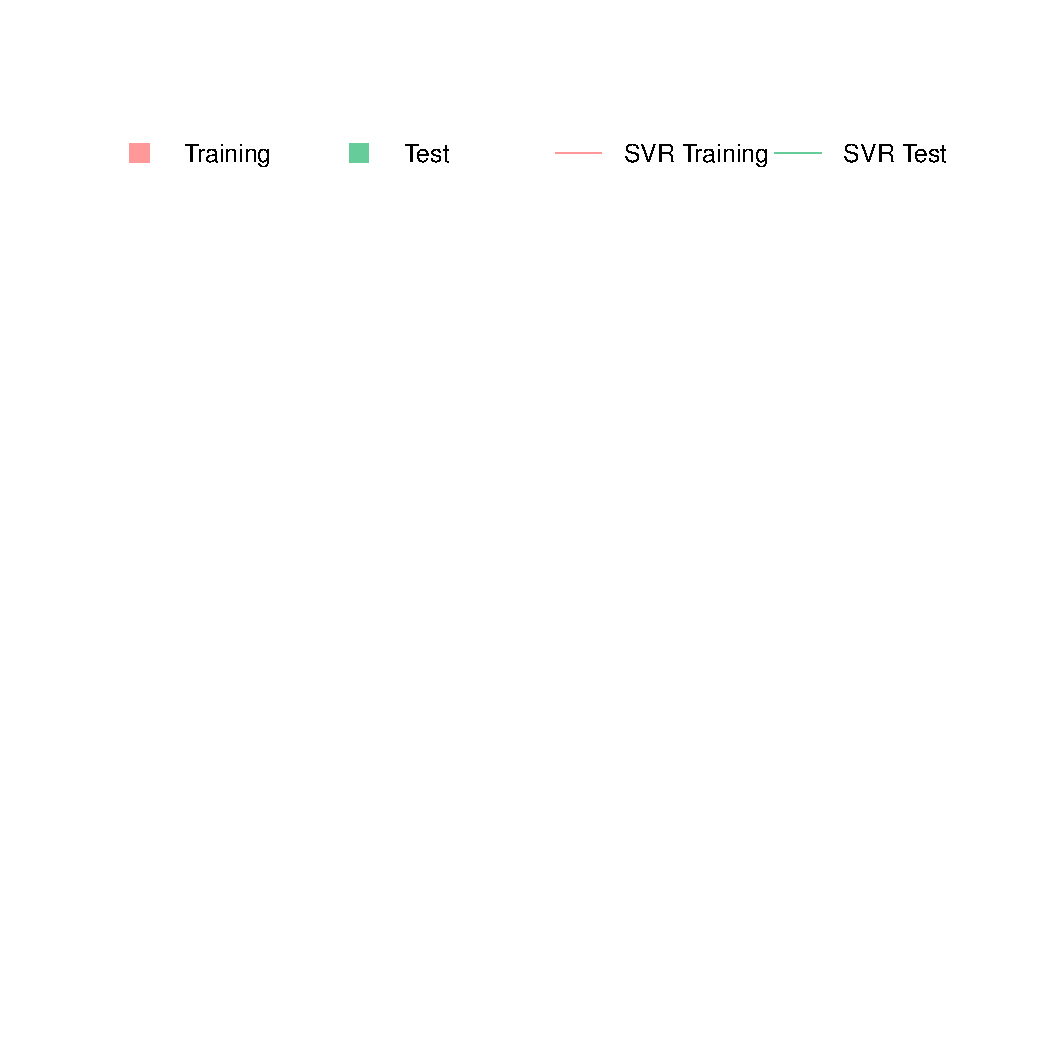
\includegraphics[height=0.35cm, width=7cm]{Box-Legend}
	\caption{Distribution of the Best \textit{Training} and \textit{Test} RSEs.}
	\label{fig:Box}
\end{figure*}

As shown in Fig. \ref{fig:Box}, both GP and GPRC have comparable training performance to the SVR. GP outperforms SVR on four of the six training sets, SVR being better on the CCUN and DLBCL datasets. GPRC has better training performance than SVR on Concrete, Wine, and BHouse, and worse performance on the other three training sets. The results of Z-test show that all these differences are significant. Considering the comparison between the two GP methods, the proposed GPRC method usually has a worse training performance than standard GP on the examined problems. While on LD50 and DLBCL, GPRC has a notably higher training error, on the other four training sets, GPRC has a slightly worse training performance than standard GP. According to the statistical test, all the differences between the two GP methods on the training performance are significant. 

The pattern on the training data is not unexpected since GPRC has an implicit objective of evolving simpler regression models. With this objective, the evolutionary process of GPRC is driven towards GP individuals having a lower value of Rademacher complexity. This objective often conflicts with the objective of a smaller training error, particularly when the candidate model overfits the training data. The conflict of these two objectives  undoubtedly leads to a worse training RSE which is the compromise made for a better generalization capacity.

\begin{figure*}[t]
	\centering
	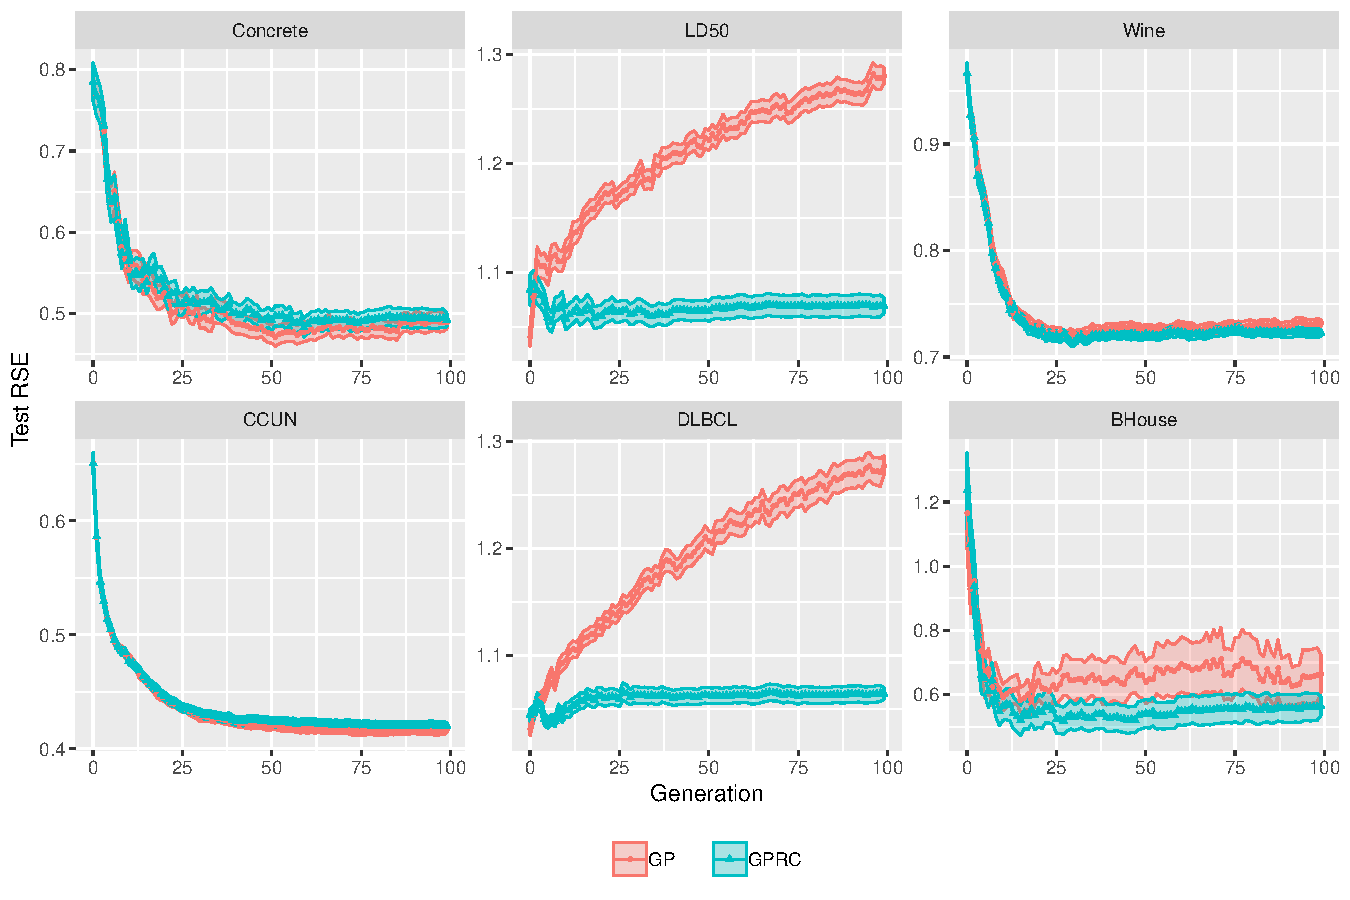
\includegraphics[height=9cm, width=13cm]{Plot}
	\caption{Evolutionary Plots of the \textit{Test} RSEs.}
	\label{fig:Plot}
\end{figure*}

\subsection{Comparing the Test Performance}
In regards to the generalization performance, which is typically more important than the training performance for a supervised learning algorithm, the proposed method GPRC has the best performance on the majority of the examined data sets. The pattern is very similar with the training set when comparing GPSR with SVR on their test performance. On four of the six test sets (except for CCUN and DLBCL) GPRC achieves a notably better generalization performance in contrast to SVR, while on the other two test sets, GPRC has a significantly worse test performance. Compared with standard GP, on four of the six test sets (LD50, DLBCL, Wine and BHouse) GPRC has better generalization performance than standard GP. On LD50 and DLBCL, GPRC achieves notably and significantly lower test RSEs than GP. This is shown by the significantly lower and shorter interquartile ranges (in green) of GPRC, which does not have any overlap with that of GP on the two test sets. On wine and DLBCL, GPRC slightly outperforms standard GP on the generalization performance. On Concrete and CCUN, GPRC has a slightly higher test error than standard GP. But no statistically significant difference has been found on the four test sets. 

An interesting pattern on the generalization performance is that on datasets where standard GP outperforms GPRC most on the training sets i.e. LD50 and DLBCL, GPRC has the most obvious generalization gain when compared to the standard GP. A possible reason for this phenomenon is that the hypothesises evolved by standard GP overfit the training set thus could not generalize well onto the test set. In this case GPRC which considers the complexity is able to evolve individuals with a better generalization performance. This is accomplished by identifying and assigning a higher fitness values to models with a lower estimated generalization error. 

\subsection{Evolutionary Plots on the Test Sets}
To examine the generalization performance of the proposed method GPRC in more detail, the evolutionary plots on the test errors over generations of the two GP methods have been presented in Fig. \ref{fig:Plot}. These plots are drawn using the test RSEs of the best-of-generation models in the two GP methods.

As shown in Fig. \ref{fig:Plot}, on three of the six dataset (LD50, DLBCL and BHouse), GPRC has a much better generalization performance than standard GP which is indicated by the large distance between the plots and the smaller band of the plot in GPRC. On the other three datasets where standard GP generalize well, GPRC has a slightly smaller test error on Concrete and Wine and a slightly higher test error on CCUN, however, the differences are not significant.

On LD50 and DLBCL, the test RSEs of GP increase dramatically after a decrease at the first several generations (2-3 generations). On BHouse, GP has an increased test error in the early stages of the evolutionary process. Meanwhile, the wide band of the test plot further indicates high fluctuation across each generations. 

On these three datasets (LD50, DLBCL and BHouse), standard GP suffers from severe overfitting while GPRC generalizes well and outperforms standard GP in the early stage of the evolutionary process. The advantage of GPRC on the generalization performance is brought by the new fitness function which takes both the training error and the model complexity into consideration. The model complexity, which is measured by the Rademacher complexity, accurately reflects the generalization performance of the GP individuals during the evolutionary process. Based on the complexity values, the new fitness function assigns a more accurate fitness value to the simpler individuals with a similar (the same or slightly smaller) training error to their more complex counterparts and leads the evolutionary process towards hypothesises with better generalization performance. 

Meanwhile, the comparable generalization performance of GPRC and standard GP on Concrete, Wine and CCUN also confirms the positive effort of the Rademacher complexity measuring the complexity of GP individuals on estimating their generalization capacity. On these three datasets where standard GP generalizes well, GPRC also generalizes well and does not have any premature convergence issues, which is a common limitation of many existing methods for solving overfitting and model complexity in GP \cite{b20}.

\subsection{A Further Examination of Program Sizes and Computational Times}

\begin{table}[t]
	\centering
	\caption{Program Size and Computational Time. }
	\scriptsize
	\begin{tabular}{|l|l|c|c|c|c|}
\hline
\multirow{2}{*}{} & \multicolumn{1}{c|}{\multirow{2}{*}{Methods}}     & \multicolumn{2}{c|}{Size (\#Nodes)}                                                                       & \multicolumn{2}{l|}{Time (Seconds)}                                                                         \\ \cline{3-6} 
                  & \multicolumn{1}{c|}{}                             & Mean                                                    & Best                                            & Mean                                                  & Best                                                \\ \hline
Concrete          & \begin{tabular}[c]{@{}l@{}}GP\\ GPRC\end{tabular} & \begin{tabular}[c]{@{}c@{}}131.46\\ 125.34\end{tabular} & \begin{tabular}[c]{@{}c@{}}61\\ 65\end{tabular} & \begin{tabular}[c]{@{}c@{}}8.89\\ 11.35\end{tabular}  & \begin{tabular}[c]{@{}c@{}}4.43\\ 5.38\end{tabular} \\ \hline
LD50              & \begin{tabular}[c]{@{}l@{}}GP\\ GPRC\end{tabular} & \begin{tabular}[c]{@{}c@{}}157.28\\ 92.74\end{tabular}  & \begin{tabular}[c]{@{}c@{}}63\\ 35\end{tabular} & \begin{tabular}[c]{@{}c@{}}2.53\\ 2.36\end{tabular}   & \begin{tabular}[c]{@{}c@{}}1.09\\ 1.12\end{tabular} \\ \hline
Wine              & \begin{tabular}[c]{@{}l@{}}GP\\ GPRC\end{tabular} & \begin{tabular}[c]{@{}c@{}}119.5\\ 110.66\end{tabular}  & \begin{tabular}[c]{@{}c@{}}49\\ 41\end{tabular} & \begin{tabular}[c]{@{}c@{}}11.49\\ 15.03\end{tabular} & \begin{tabular}[c]{@{}c@{}}4.41\\ 6.86\end{tabular} \\ \hline
CCUN              & \begin{tabular}[c]{@{}l@{}}GP\\ GPRC\end{tabular} & \begin{tabular}[c]{@{}c@{}}117.12\\ 103.9\end{tabular}  & \begin{tabular}[c]{@{}c@{}}29\\ 25\end{tabular} & \begin{tabular}[c]{@{}c@{}}4.71\\ 6.3\end{tabular}    & \begin{tabular}[c]{@{}c@{}}1.71\\ 1.7\end{tabular}  \\ \hline
DLBCL             & \begin{tabular}[c]{@{}l@{}}GP\\ GPRC\end{tabular} & \begin{tabular}[c]{@{}c@{}}135.56\\ 76.5\end{tabular}   & \begin{tabular}[c]{@{}c@{}}13\\ 5\end{tabular}  & \begin{tabular}[c]{@{}c@{}}5.88\\ 5.77\end{tabular}   & \begin{tabular}[c]{@{}c@{}}1.82\\ 1.85\end{tabular} \\ \hline
BHouse            & \begin{tabular}[c]{@{}l@{}}GP\\ GPRC\end{tabular} & \begin{tabular}[c]{@{}c@{}}146.0\\ 121.48\end{tabular}  & \begin{tabular}[c]{@{}c@{}}67\\ 35\end{tabular} & \begin{tabular}[c]{@{}c@{}}4.68\\ 5.37\end{tabular}   & \begin{tabular}[c]{@{}c@{}}2.25\\ 1.73\end{tabular} \\ \hline
\end{tabular}
\label{tab:cputimeandsize}
\end{table}

To understand how the new fitness function influences the size of individuals and the computational cost of GP, Table \ref{tab:cputimeandsize} shows the average (mean) and smallest (best) program size in terms of the number of nodes of the $100$ best-of-run models in the two GP methods. Note that the size of the GP individuals can roughly reflect the complexity of the program sizes to some extent, although structural and functional complexity are not equivalent. The overall computational cost of the GP runs in the two GP methods is also compared with respect to the average (mean) and the shortest (best) running time for one GP run.

It is clear that GPRC generally evolves the simplest regression models, which are notable and significantly smaller than the models evolved by standard GP in all the examined datasets, particularly on LD50 and DLBCL, where standard GP overfits the training sets severely. The oversized individuals are typically overcomplex and have more space to incorporate information that is specific for the training set and could not generalize well. GPRC evolves model which are smaller in size and could generalize better.

On most of the datasets, GPRC has a higher computation cost compared to standard GP, which is caused as a result of measuring the complexity of individuals. However, the marginally increased computational time, which usually is less than 5 seconds is still affordable and does not make a notable difference. An interesting finding is that the computational time of GPRC is slightly smaller than that of standard GP on LD50 and DLBCL. The underlying reason is that the significantly smaller individuals cost less to evaluate compared to their larger counterparts in standard GP. This is compensation for the measuring and managing the model complexity.  


\section{Conclusions and Future Work}
\label{se:conclu}
This work proposed a new GP method to tackle the open problem of generalization in GP for symbolic regression. The objectives of this paper have been accomplished by incorporating a reliable complexity measure of GP individuals which is capable of providing a accurate estimation of their generalization ability. The new evaluation method based on the Rademacher complexity measure drives the evolutionary process of GPRC toward functionally and structurally simpler models that have better generalization performance. The experimental results confirm that the proposed method is effective in reducing the overfitting trend in GP without leading to premature convergence. This is the very first work  investigating and confirming the effectiveness of Rademacher complexity to improve the generalization ability of GP for symbolic regression.

In the near future, we will further develop GPRC to improve the generalization of GP. The first work is to have a more accurate measure of the complexity of GP individuals by using gradient descent to maximise the correlation with $\sigma$ since the current version is taking the average complexity across a number of observations. Another area of development to improve GPRC would be the removal of the parameter $\alpha$ which is being used to increase the pressure when overfitting occurs since this parameter requires a lengthy tuning process. We will introduce an adaptive version of GPRC which will detect overfitting happening and increase the pressure put on the complexity accordingly. Finally, an Evolutionary Multi-objective Optimization (EMO) algorithm, with the training error as the first objective and the Rademacher complexity as the second.


% Reference block

\begin{thebibliography}{00}

\bibitem{b1} T. Dietterich, “Overfitting and undercomputing in machine learning,” ACM Computing Surveys, vol. 27, no. 3, pp. 326--327, 1995.

\bibitem{b2} V. Vapnik, “Principles of risk minimization for learning theory,” Advances in neural information processing systems, pp. 831--838, 1992.

\bibitem{b3} J. R. Koza. "Genetic programming: on the programming of computers by means of natural selection", volume 1. MIT press, 1992.

\bibitem{b4} “Genetic programming II: Automatic discovery of reusable programs,” Computers and Mathematics with Applications, vol. 29, no. 3, p. 115, 1995.

\bibitem{b5} Q. Chen, B. Xue, L. Shang, and M. Zhang, “Improving Generalisation of Genetic Programming for Symbolic Regression with Structural Risk Minimisation,” Proceedings of the 18th annual conference on Genetic and Evolutionary Computation Conference (GECCO 2016), pp. 709--716.

\bibitem{b6} E. Vladislavleva, G. Smits, and D. D. Hertog, “Order of Nonlinearity as a Complexity Measure for Models Generated by Symbolic Regression via Pareto Genetic Programming,” IEEE Transactions on Evolutionary Computation, vol. 13, no. 2, pp. 333--349, 2009.

\bibitem{b7} L. Vanneschi, M. Castelli, and S. Silva, “Measuring bloat, overfitting and functional complexity in genetic programming,” Proceedings of the 12th annual conference on Genetic and evolutionary computation (GECCO 2010), pp. 877--884.

\bibitem{b8} T. Soule and J. A. Foster, “Effects of Code Growth and Parsimony Pressure on Populations in Genetic Programming,” Evolutionary Computation, vol. 6, no. 4, pp. 293--309, 1998.

\bibitem{b9} S. Luke and P. Liviu, “Lexicographic Parsimony Pressure,” Proceedings of the 4th Annual Conference on Genetic and Evolutionary Computation, 2002.

\bibitem{b10} N. Le, H. N. Xuan, A. Brabazon, and T. P. Thi, “Complexity measures in Genetic Programming learning: A brief review,” 2016 IEEE Congress on Evolutionary Computation (CEC), pp. 3--4. 2016.

\bibitem{b11} D. Anguita, A. Ghio, L. Oneto, and S. Ridella, “Structural Risk Minimization and Rademacher Complexity for Regression,” European Symposium on Artificial Neural Networks, pp. 55--60, 2012. 

\bibitem{b12} O. Bousquet and D. J. L. Herrmann, “On the Complexity of Learning the Kernel Matrix,” Conference and Workshop on Neural Information Processing Systems: Advances in Neural Information Processing Systems 31, pp. 1--5, 2003. 

\bibitem{b13} V. Koltchinskii, “Penalized Empirical Risk Minimization and Model Selection Problems,” Lecture Notes in Mathematics Oracle Inequalities in Empirical Risk Minimization and Sparse Recovery Problems, pp. 99–119, 2011.

\bibitem{b14} J. R. Koza and R. Poli, “Search methodologies: Introductory tutorials in optimization and decision support techniques - Chapter 5: Genetic Programming.”

\bibitem{b15} V. Vapnik, E. Levin, and Y. Le Cun. "Measuring the VC-dimension of a learning machine", 1994.

\bibitem{b16} Q. Chen, B. Xue and M. Zhang, “Improving Generalisation of Genetic Programming for Symbolic Regression with Angle-Driven Geometric Semantic Operators,” IEEE Transactions on Evolutionary Computation, 2018

\bibitem{b17} Q. Chen, M. Zhang and B. Xue, “Structural Risk Minimisation-Driven Genetic Programming for Enhancing Generalisation in Symbolic Regression,” IEEE Transactions on Evolutionary Computation, 2018

\bibitem{b18} F.  A.  A.  Motta,  J.  M.  D.  Freitas,  F.  R.  D.  Souza,  H.  S.  Bernardino,I.  L.  D.  Oliveira,  and  H.  J.  C.  Barbosa,  “A  hybrid  grammar-basedgenetic programming for symbolic regression problems,” in 2018 IEEE Congress on Evolutionary Computation (CEC), 2018, pp. 1--8

\bibitem{b19} Z.  Huang,  J.  Zhong,  W.  Liu,  and  Z.  Wu,  “Multi-population  genetic programming  with  adaptively  weighted  building  blocks  for  symbolicregression,” in Proceedings of the Genetic and Evolutionary Computation Conference Companion (GECCO), pp. 266--267, 2018.

\bibitem{b20} S. Luke and L. Panait, “Fighting bloat with nonparametric parsimony pressure,” in International Conference on Parallel Problem Solving from Nature (PPSN). 2002, pp. 411--421.

\bibitem{b21} M. Lichman. 2013. UCI Machine Learning Repository. (2013). http://archive.ics.uci.edu/ml 

\bibitem{b22} Archetti, F., Lanzeni, S., Messina, E., Vanneschi, L.: Genetic programming for computational pharmacokinetics in drug discovery and development. Genetic Programming and Evolvable Machines 8(4), 413–432 (2007)

\bibitem{b23} Rosenwald, A., Wright, G., Chan, W.C., Connors, J.M., Campo, E., Fisher, R.I., GascoyneR.D., Muller-Hermelink, H.K., Smeland, E.B., Giltnane, J.M., et al.: The use of moleculaprofiling to predict survival after chemotherapy for diffuse large-b-cell lymphoma. New England Journal of Medicine 346 (25), (2002)

\bibitem{b24} Sean Luke, Liviu Panait, Gabriel Balan, Sean Paus, Zbigniew Skolicki, Elena
Popovici, Keith Sullivan, Joseph Harrison, Jeff Bassett, Robert Hubley, et al. 2004.
A java-based evolutionary computation research system. Online (March 2004)
\url{http://cs.gmu.edu/~eclab/projects/ecj} (2004).

\bibitem{b25} David Meyer and FH Technikum Wien. 2001. Support vector machines. R News
1, 3 (2001), pp. 23-–26.

\bibitem{b26} P. L. Bartlett and S. Mendelson, “Rademacher and Gaussian Complexities: Risk Bounds and Structural Results,” Lecture Notes in Computer Science Computational Learning Theory, pp. 224–240, 2001.

\bibitem{b27} P. L. Bartlett, O. Bousquet, and S. Mendelson, “Localized Rademacher Complexities,” Lecture Notes in Computer Science Computational Learning Theory, pp. 44–58, 2002.

\end{thebibliography}

\end{document}
